\documentclass{article}

\usepackage{amsmath, amsthm, amssymb, amsfonts}
\usepackage{thmtools}
\usepackage{graphicx}
\usepackage{setspace}
\usepackage{geometry}
\usepackage{float}
\usepackage{hyperref}
\usepackage[utf8]{inputenc}
\usepackage[english]{babel}
\usepackage{framed}
\usepackage[dvipsnames]{xcolor}
\usepackage{tcolorbox}
\usepackage{ dsfont }


\colorlet{LightGray}{White!90!Periwinkle}
\colorlet{LightOrange}{Orange!15}
\colorlet{LightGreen}{Green!15}

\graphicspath{ {./pictures/} }

\newcommand{\HRule}[1]{\rule{\linewidth}{#1}}

% ------------------------------------------------------------------------------

\begin{document}

% ------------------------------------------------------------------------------
% Cover Page and ToC
% ------------------------------------------------------------------------------

\title{ \normalsize \textsc{}
		\\ [2.0cm]
		\HRule{1.5pt} \\
		\LARGE \textbf{\uppercase{Mathe Hausübung Nr. 3}
		\HRule{2.0pt} \\ [0.6cm] \LARGE{Sebastian Steitz, Hannes Albert} \vspace*{10\baselineskip}}
		}
\date{Mai 2022}
\author{\textbf{} \\ 
		Gruppe: 6 \\
		Tutor: Zidane Bührmann }

\maketitle
\newpage

\setlength\leftskip{1cm}
\section{H3.1}
\bigskip
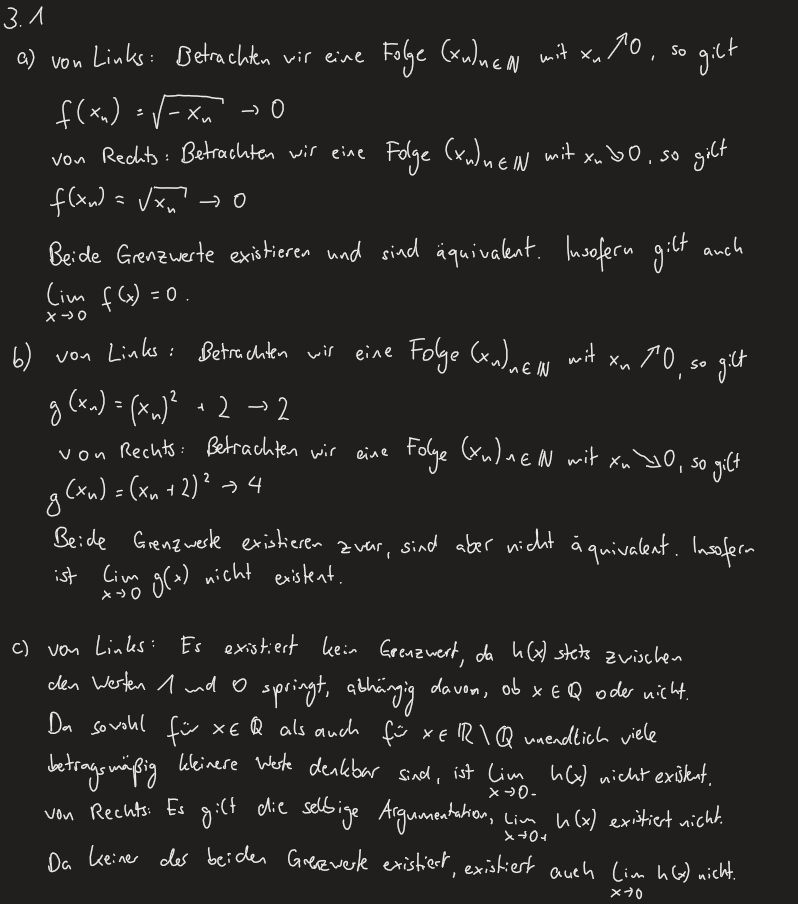
\includegraphics[scale=0.6]{h3_1} 

\section{H3.2}
\bigskip
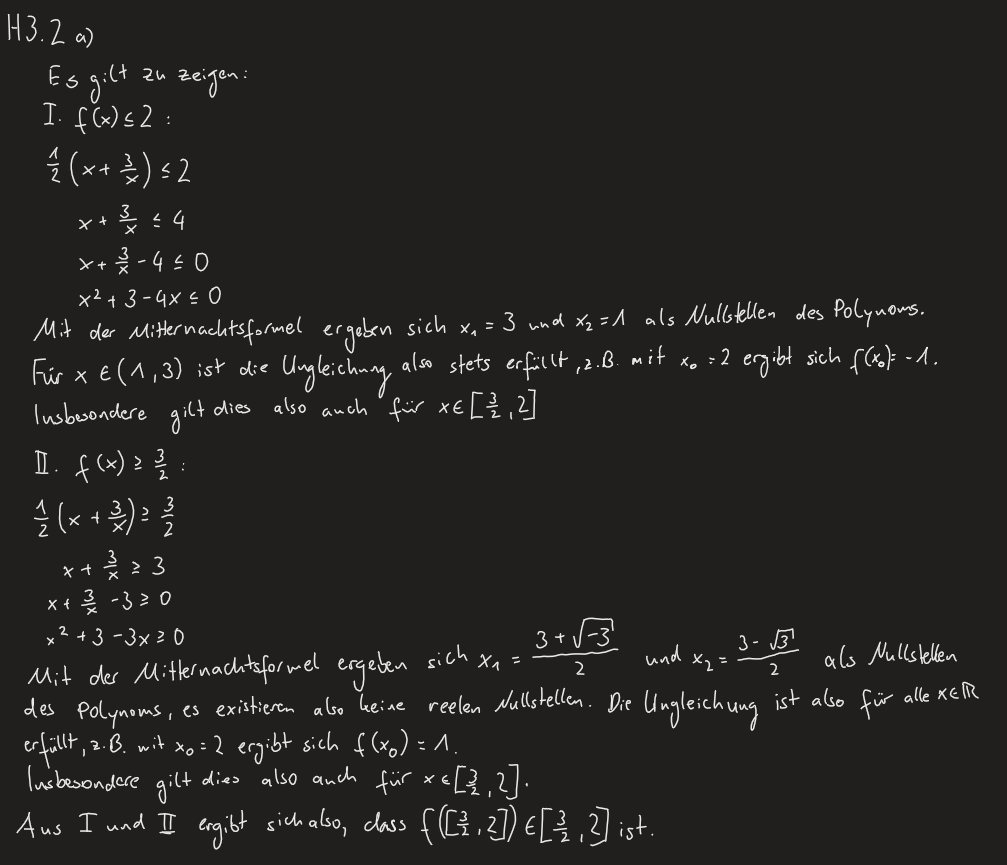
\includegraphics[scale=0.5]{h3_2a} 

\newpage
\noindent b) \\
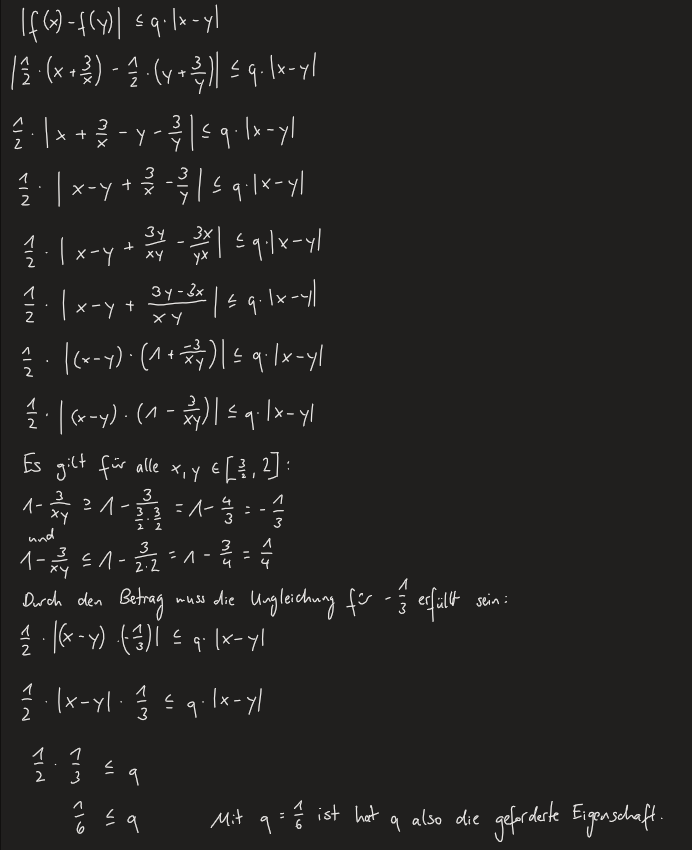
\includegraphics[scale=0.5]{h2_2b} \\ 
\bigskip
\noindent c) \\ 
Wir setzen $\sqrt{3}$ in unsere Funktion ein: 
\begin{align*}
    f(\sqrt{3}) = \frac{1}{2} * (\sqrt{3} + \frac{3}{\sqrt{3}}) 
                = \frac{1}{2} * 2 * \sqrt{3} 
                = \sqrt{3}
\end{align*}
Damit gilt nach 5.6.22 (Banach'scher Fixpunktssatz), dass es sich bei $\sqrt{3}$ 
um den einigsten Fixpunkt der Funktion handelt.
\newpage
\noindent d) \\ 
Zunächst berechnen wir unser $x_1$: 
\begin{align*}
    | x_1 - \sqrt{3} | < 0,001  \indent \indent | + \sqrt{3} \\ 
    x_1 < 0,001 + \sqrt{3} \\ 
    x_1 < 0,001 + 1,73 \\ 
    x_1 < 1,733 \approx \frac{7}{4} \\ 
\end{align*}
Dies setzen wir in die Appriori-Abweichung inklusive des Wertes für q aus b) ein: 
\begin{align*}
    | x_n - \sqrt{3}| \leq \frac{(\frac{1}{6})^n}{1 - \frac{1}{6}} * |x_1 - x_0| \\ 
                       = \frac{1}{6^n} * \frac{1}{\frac{5}{6}} * |x_1 - x_0| \\
                       = \frac{6}{5 * 6 ^ n} * |x_1 - x_0| \\
                       = \frac{1}{5 * 6 ^ {n - 1}} * |x_1 - x_0| \\
\end{align*}
Wir wählen unser $x_0$ als $\frac{3}{4}$:

\begin{align*}
    \frac{1}{5 * 6^{n - 1}} * |\frac{7}{4} - \frac{3}{4}| = \frac{1}{5 * 6^{n - 1}} * 1 \\  
    = \frac{1}{5 * 6^{n - 1}} 
\end{align*}
Für $x_4$ erhalten wir durch einsetzen in die Formel: 
\[
    |x_4 - \sqrt{3}| = \frac{1}{5 * 6^{4 - 1}} = \frac{1}{5 * 6^{3}} = 0,000\overline{925} \approx 0,001
\]
$x_4$ hat somit den Wert $x_4 = \sqrt{3}$ + 0,001 = 1,743, während $\sqrt{3}$ = 1,732. Somit sind die 
beiden Werte sich ziemlich ähnlich.

\section{H3.3}

\noindent a) \\ 
Betreachten wir exp(x) zunächst für x $>$ 0: 
\begin{align*}
    exp(x) = \sum_{k = 0}^{\infty} \frac{x^k}{k!} > 1 + \sum_{k = 1}^{\infty} \frac{0^k}{k!} = 1
\end{align*}
Da für alle x $<$ 0 gilt: exp(-x) = $\frac{1}{exp(x)}$ $>$ 0, lässt sich schließen, dass für 
alle x $\in \mathds{R}$ exp(x) $>$ 0.
Seien nun x, y $\in \mathds{R}$ mit x $>$ y: 
\[
    1 < exp(x - y) = \frac{exp(x)}{exp(y)}
\]
Da exp strikt positiv ist können wir hier Umformen ohne die Ungleichung verändern zu müssen. 
Smit erhalten wir exp(x) $<$ exp(y) und es ist gezeigt, dass exp streng monoton wächst.
Für die Stetigkeit von exp gilt folgendes: 
$\lim\limits_{x \to 0+}$ exp(x) = 1 \\ 
Dann gilt für $\lim\limits_{x \to 0-}$ exp = $\lim\limits_{x \to 0+}$ exp(-x) = 1

Sei $x_0 \in \mathds{R}$:
\begin{align*}
   \noindent \lim\limits_{x \to x_0} exp(x) = \lim\limits_{x \to 0} exp(x_0 + x) \\
                                   = exp(x_0) * \lim\limits_{x \to 0} exp(x)
                                   = exp(x_0) * 1
                                   = exp(x_0)
\end{align*}
Somit wurde die Stetigkeit für exp gezeigt.

\noindent b) \\ 
Wir wissen aus Beispiel 5.7.8, dass $\lim\limits_{x \to \infty}$ exp(x) = $\infty$ und 
$\lim\limits_{x \to - \infty}$ exp(x) = 0. Mithhilfe des Zwischenwertsatzes erhalten wir 
somit für jedes y $\in \mathds{R}$ folgendes: \\ 
Wir wählen a, b $\in$ (0, $\infty$) und y $\in$ [exp(a), exp(b)]. Laut dem Zwischenwertsatz haben wir somit eine 
Garantie für die existenz eines Elements $x_0$ mit exp($x_0$) = y.
Dies gibt uns die Surjektivität.
Aus dem strengen Wachstum der Funktion folgt schon, dass für f(x) = f(y), x = y gelten muss. Somit ist die Injektivität gezeigt und 
die Funktion ist somit bijektiv.
\end{document}

